%% Seção 1: A Mente como Totalidade de Processos Interdependentes

\chapter{A Mente como Totalidade de Processos Interdependentes e a Importância de Nomear}

\epigrafe{Os limites da minha linguagem significam os limites do meu mundo.}{Ludwig Wittgenstein, \textit{Tractatus Logico-Philosophicus}}

\textbf{1.} O mundo psiquiátrico é a totalidade dos fatos sobre a linguagem, cognição e emoção, onde nomear é dar existência.

\section{A psiquiatria e os fatos internos}

\textbf{1.1} A psiquiatria trata de fatos internos, ou seja, da organização mental e emocional do paciente, que se constroem através da nomeação e da linguagem.

\begin{tese}
Se a mente humana é composta por cognição, emoção e linguagem, e se nomear é dar existência, então esses processos são interdependentes, e a linguagem é fundamental na construção do self.
\end{tese}

\begin{hipotese}[title=Hipótese 1.1.1 (Condicional)]
Se nomeamos nossas experiências internas, então organizamos e damos forma à nossa cognição e emoção.
\end{hipotese}

\begin{prova}
Se não pudéssemos nomear nossas experiências, não poderíamos compreendê-las ou comunicá-las, o que levaria a uma desorganização interna e isolamento.
\end{prova}

\begin{aforismo}
As coisas só existem quando nomeadas; o ser nasce na palavra.
\end{aforismo}

\section{A linguagem como veículo de expressão e construção}

\textbf{1.2} A linguagem é o veículo pelo qual o mundo interno se expressa no mundo externo e se constrói através da ação comunicativa.

\begin{tese}
Se a linguagem é o meio pelo qual a mente organiza seus processos internos e constrói o self, então a comunicação autêntica é essencial para a compreensão de si mesmo.
\end{tese}

\begin{hipotese}[title=Hipótese 1.2.1 (Condicional)]
Se engajamos em uma ação comunicativa genuína, então promovemos a reflexão crítica e a autodescoberta.
\end{hipotese}

\begin{referencia}[title=Referência a Habermas]
De acordo com a teoria da ação comunicativa de Habermas, a comunicação orientada para o entendimento mútuo permite que os indivíduos revelem e questionem suas próprias premissas, promovendo a emancipação.
\end{referencia}

\begin{aforismo}
Na palavra compartilhada, o eu se revela e se constrói.
\end{aforismo}

\section{Coerência e desorganização da linguagem}

\textbf{1.3} A coerência ou desorganização da linguagem reflete a estruturação ou falha da cognição, influenciada pelos afetos.

\begin{tese}
Se os afetos influenciam diretamente nossa capacidade de agir e pensar (conforme Spinoza), então a linguagem que usamos reflete nossos estados emocionais e cognitivos.
\end{tese}

\begin{hipotese}[title=Hipótese 1.3.1 (Condicional)]
Se compreendemos e nomeamos nossos afetos, então podemos reorganizar nossa cognição e linguagem de forma mais coerente.
\end{hipotese}

\begin{referencia}[title=Referência a Spinoza]
Spinoza argumenta que os afetos são expressões da potência do ser; compreendê-los aumenta nossa capacidade de agir de forma autônoma.
\end{referencia}

\begin{aforismo}
Nomear o afeto é dominar a tempestade interna.
\end{aforismo}

\section{Estados emocionais e expressões de afetos}

\textbf{1.4} Os estados emocionais manifestam-se na linguagem como expressões de afetos e intenções, conduzindo à autonomia de existir.

\begin{tese}
Se ao nomear e compreender nossos afetos ganhamos autonomia (Spinoza), então a linguagem é o instrumento que nos conduz a uma existência autêntica.
\end{tese}

\begin{hipotese}[title=Hipótese 1.4.1 (Condicional)]
Se utilizamos a linguagem para expressar e refletir sobre nossos afetos, então nos aproximamos da autonomia de existir, transcendendo pensamentos automáticos.
\end{hipotese}

\begin{aforismo}
Na palavra intencional, a liberdade encontra morada.
\end{aforismo}

\section{Dinâmicas de poder e contextos socioculturais}

\textbf{1.5} As dinâmicas de poder, os contextos socioculturais e as estruturas subjetivas afetam profundamente a maneira como a linguagem se organiza, influenciando a construção do self.

\begin{tese}
Se a linguagem é moldada pelo contexto sociocultural e pelas dinâmicas de poder, então compreender essas influências é essencial para a construção de uma identidade autêntica e autônoma.
\end{tese}

\begin{hipotese}[title=Hipótese 1.5.1 (Silogismo)]
\textbf{Premissa maior:} A linguagem é influenciada pelo contexto sociocultural e dinâmicas de poder.\\
\textbf{Premissa menor:} O self é construído através da linguagem.\\
\textbf{Conclusão:} Logo, o self é influenciado pelo contexto sociocultural e dinâmicas de poder.
\end{hipotese}

\begin{aforismo}
Para ser autêntico, é preciso reconhecer as vozes que ecoam em nossas palavras.
\end{aforismo}

%% DIAGRAMA DA SEÇÃO 1
\section*{Diagrama Representativo: Interdependência Mental}

\begin{center}
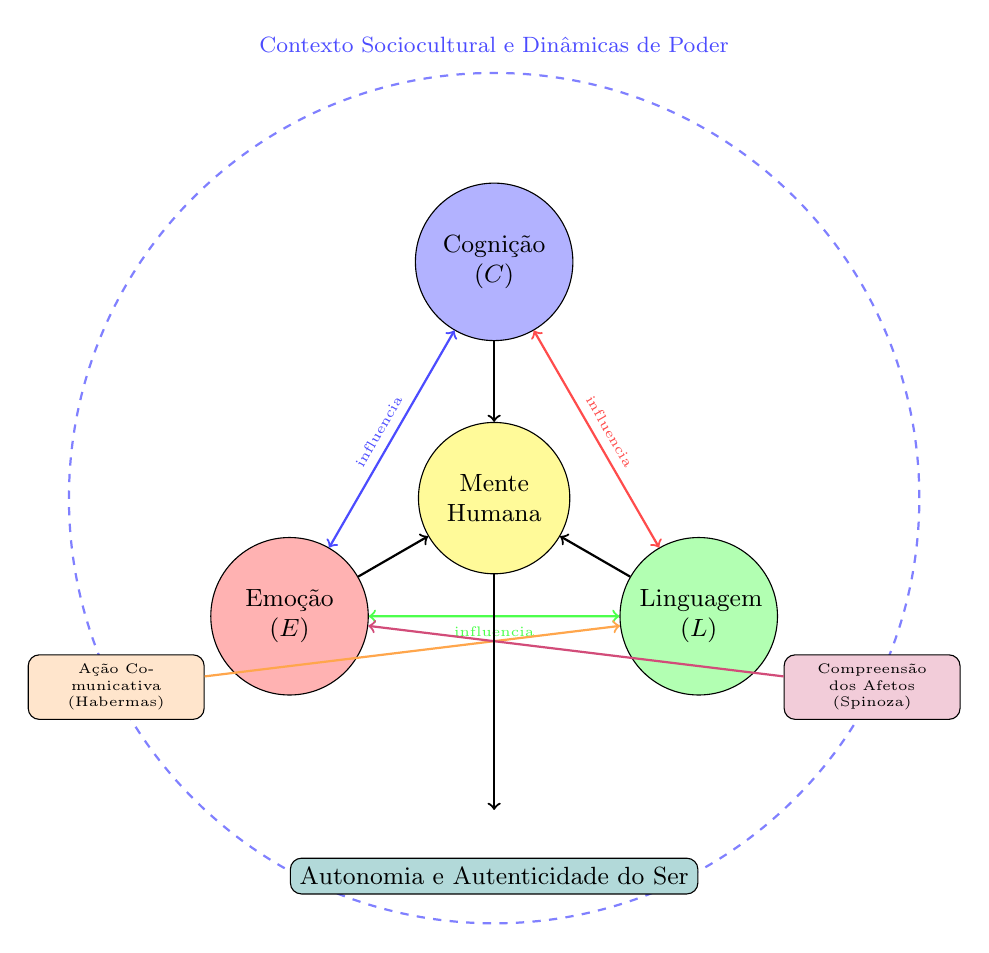
\begin{tikzpicture}[scale=1.2, every node/.style={font=\small}]
    % Círculo externo - Contexto Sociocultural
    \draw[thick, dashed, blue!50] (0,0) circle (4.5cm);
    \node[blue!70, font=\footnotesize] at (0,4.8) {Contexto Sociocultural e Dinâmicas de Poder};

    % Triângulo central
    \coordinate (C) at (90:2.5);   % Cognição (topo)
    \coordinate (E) at (210:2.5);  % Emoção (esquerda)
    \coordinate (L) at (330:2.5);  % Linguagem (direita)

    % Nós principais
    \node[draw, circle, fill=blue!30, minimum size=2cm, text width=1.5cm, align=center] (cog) at (C) {Cognição\\$(C)$};
    \node[draw, circle, fill=red!30, minimum size=2cm, text width=1.5cm, align=center] (emo) at (E) {Emoção\\$(E)$};
    \node[draw, circle, fill=green!30, minimum size=2cm, text width=1.5cm, align=center] (lin) at (L) {Linguagem\\$(L)$};

    % Centro - A Mente
    \node[draw, circle, fill=yellow!40, minimum size=1.8cm, text width=1.5cm, align=center] (mente) at (0,0) {Mente\\Humana};

    % Setas bidirecionais entre os componentes
    \draw[thick, <->, blue!70] (cog) -- node[above, sloped, font=\tiny] {influencia} (emo);
    \draw[thick, <->, green!70] (emo) -- node[below, sloped, font=\tiny] {influencia} (lin);
    \draw[thick, <->, red!70] (lin) -- node[above, sloped, font=\tiny] {influencia} (cog);

    % Setas para o centro
    \draw[thick, ->] (cog) -- (mente);
    \draw[thick, ->] (emo) -- (mente);
    \draw[thick, ->] (lin) -- (mente);

    % Fluxos externos
    \node[draw, rounded corners, fill=orange!20, font=\tiny, text width=2cm, align=center] (hab) at (-4,-2) {Ação Comunicativa\\(Habermas)};
    \node[draw, rounded corners, fill=purple!20, font=\tiny, text width=2cm, align=center] (spi) at (4,-2) {Compreensão\\dos Afetos\\(Spinoza)};

    \draw[thick, ->, orange!70] (hab) -- (lin);
    \draw[thick, ->, purple!70] (spi) -- (emo);

    % Resultado
    \node[draw, rounded corners, fill=teal!30, font=\small] at (0,-4) {Autonomia e Autenticidade do Ser};
    \draw[thick, ->] (mente) -- (0,-3.3);
\end{tikzpicture}
\end{center}

\begin{sintese}[title=Síntese Final da Seção 1]
A mente humana é uma totalidade de processos interdependentes, onde cognição, emoção e linguagem se entrelaçam em um fluxo contínuo. Nomear é dar existência; é através da linguagem que construímos nossa identidade, organizamos nossos pensamentos e compreendemos nossos afetos. A ação comunicativa autêntica, conforme Habermas, permite que revelemos e reconstruamos nosso self, promovendo a reflexão crítica e a autonomia. Segundo Spinoza, compreender e nomear nossos afetos aumenta nossa potência de agir, conduzindo-nos a uma existência mais livre e consciente.

As dinâmicas de poder e os contextos socioculturais moldam a maneira como a linguagem se organiza, influenciando a construção do self. Reconhecer essas influências é essencial para alcançar a autenticidade e a autonomia. A linguagem, portanto, não é apenas um meio de comunicação, mas o fundamento sobre o qual a mente se ergue, influenciando e sendo influenciada pelos processos cognitivos e emocionais.
\end{sintese}

%% Representação Matemática
\subsection*{Formalização Matemática}

A interdependência entre cognição ($C$), emoção ($E$) e linguagem ($L$) pode ser formalizada como um sistema de equações diferenciais acopladas:

\begin{align}
\frac{dC}{dt} &= f_C(C,E,L) \\
\frac{dE}{dt} &= f_E(C,E,L) \\
\frac{dL}{dt} &= f_L(C,E,L)
\end{align}

Onde as funções $f_C$, $f_E$ e $f_L$ representam a taxa de mudança de cada componente em relação aos outros, capturando a interdependência dinâmica do sistema.

\nextpage
